%%
%%
\documentclass[12pt]{book}
\usepackage{amsfonts}
\usepackage{amsmath}
\usepackage{amssymb}
\usepackage{graphicx}
\usepackage{hyperref}
\usepackage{verbatim}
\usepackage{float}
\setlength{\textheight}{10in}
\setlength{\textwidth}{7.4in}
\setlength{\topmargin}{-0.75in}
\setlength{\oddsidemargin}{-0.5in}
\setlength{\evensidemargin}{-0.5in}
\setlength{\parskip}{0.15in}
\setlength{\parindent}{0in}



\begin{document}


\vspace{-1.0in}\begin{center}
\Large{MCV4UR : Advanced Placement Calculus and Vectors }

\Large{Assignment \#3}


\end{center}

%\medskip

\vspace{0.015in}\hrulefill\ 

\textbf{Reference Declaration} %  Fill in your Reference Declarations in this section before your submit your assignment.

Complete the Reference Declaration section below in order for your assignment to be graded.

If you used any references beyond the course text and lectures (such as other texts, discussions with colleagues or online resources), indicate this information in the space below.  If you did not use any aids, state this in the space provided. 

Be sure to cite appropriate theorems throughout your work. You may use shorthand for well-known theorems like the MVT, IVT, etc. 

Note: Your submitted work must be \textbf{your original work}. 

Family Name: Do\\%Family Name Here
First Name: Kien%First Name Here

Declared References: Discussion with my dad on question 1.

% Type your references here.
% You can use as many lines as required.

\vspace{0.015in}\hrulefill\ 

\newpage

%%%%%%%%%%%% PROBLEMS START HERE

\begin{enumerate}

%% PROBLEM 1
\item Prove that the length of the portion of any tangent line to the astroid $x^{\frac{2}{3}} + y^{\frac{2}{3}} = a^{\frac{2}{3}} \,\,\,(a \in \mathbb{R}^+)$ cut off by the coordinate axes is constant.\\

\textbf{Solution:}\\
Determine the derivative of $x^{\frac{2}{3}} + y^{\frac{2}{3}} = a^{\frac{2}{3}}$.
\setcounter{equation}{0}
\begin{align}
    a^{\frac{2}{3}} &= x^{\frac{2}{3}} + y^{\frac{2}{3}} \\
    \dfrac{d}{dx} \left(a^{\frac{2}{3}}\right) &= \dfrac{d}{dx} \left(x^{\frac{2}{3}} + y^{\frac{2}{3}}\right) \\
    0 &= \dfrac{2}{3} x^{-\frac{1}{3}} + \dfrac{2}{3} y^{-\frac{1}{3}}y' \\
    0 &= \dfrac{2}{3\sqrt[3]{x}} + \dfrac{2}{3\sqrt[3]{y}}y' \\
    y' &= -\dfrac{2}{3\sqrt[3]{x}} \times \dfrac{3\sqrt[3]{y}}{2} \\
    y' &= -\dfrac{\sqrt[3]{y}}{\sqrt[3]{x}}
\end{align}
The tangent line to the asteroid must be a linear function, therefore, it can be represented in the general form $y = ax + b$. Since the coefficient of $x$ is the tangent line's slope, we can sub in $y'$ from line (6) into the tangent function. Since $y'$ is the slope of the asteroid at some coordinate $x_0$ and $y_0$, we have, $$y = -\dfrac{\sqrt[3]{y_0}}{\sqrt[3]{x_0}}\,x + b$$
\begin{minipage}{0.5\textwidth}
    Consider Figure 1 on the right. This is a sketch of the asteroid in quadrant 1 with a tangent line on $(x_0, y_0)$ and is cut off by the coordinate axes. Since we have determined the equation of the tangent line to be\\ $$y = -\dfrac{\sqrt[3]{y_0}}{\sqrt[3]{x_0}}\,x + b$$\\ we can determine $b$ by subbing in $x=x_0$ and $y=y_0$.
\end{minipage}
\begin{minipage}{0.5\textwidth}
    \begin{figure}[H] %% figure 1
    \centering{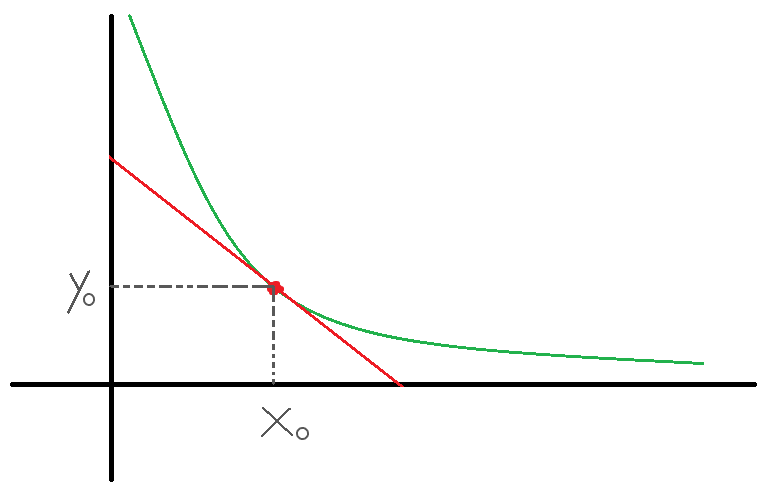
\includegraphics[width=8cm]{Q1Image.png}}
    \caption{Tangent line at ($x_0, y_0$)}
    \end{figure}
\end{minipage}\\\\
So, let's sub in $x=x_0$ and $y=y_0$ to determine $b$.
\begin{align}
    y &= -\dfrac{\sqrt[3]{y_0}}{\sqrt[3]{x_0}}\,x + b \\
    (y_0) &= -\dfrac{\sqrt[3]{y_0}}{\sqrt[3]{x_0}}\,(x_0) + b \\
    b &= y_0 + \dfrac{\sqrt[3]{y_0}}{\sqrt[3]{x_0}}\,(x_0) \\
    b &= y_0 + y_0^{\frac{1}{3}} \, x_0^{\frac{2}{3}}
\end{align}\\

But, recall that the equation of the asteroid is $x^{\frac{2}{3}} + y^{\frac{2}{3}} = a^{\frac{2}{3}}$, therefore, $x^{\frac{2}{3}} = a^{\frac{2}{3}} - y^{\frac{2}{3}}$.\\\\
Since the point $(x_0,y_0)$ is on the tangent line as well as the asteroid, we can sub in $x_0^{\frac{2}{3}} = a^{\frac{2}{3}} - y_0^{\frac{2}{3}}$ into line (10) above.
\begin{align}
    b &= y_0 + y_0^{\frac{1}{3}} \, x_0^{\frac{2}{3}} \\
    b &= y_0 + y_0^{\frac{1}{3}} \, \left(a^{\frac{2}{3}} - y_0^{\frac{2}{3}}\right) \\
    b &= y_0 + y_0^{\frac{1}{3}}a^{\frac{2}{3}} - y_0^{\frac{1}{3}}y_0^{\frac{2}{3}} \\
    b &= y_0 + y_0^{\frac{1}{3}}a^{\frac{2}{3}} - y_0 \\
    b &= y_0^{\frac{1}{3}}a^{\frac{2}{3}}
\end{align}
Therefore, we have that the tangent equation is $y = -\dfrac{\sqrt[3]{y_0}}{\sqrt[3]{x_0}}\,x + y_0^{\frac{1}{3}}a^{\frac{2}{3}}$.\\

We know that the tangent line will intersect the $x$-axis and the $y$-axis, forming a right angled triangle. The adjacent sides of this triangle are the distance from (0,0) to the intersection point on the $x$-axis and the $y$-axis and the hypotenuse is the length of the tangent cut off by the coordinate axes. We can determine the adjacent lengths by letting $y=0$ and $x=0$ in the linear tangent line in order to determine $x$ and $y$, respectively.\\

Determine $y$ when $x=0$.
\begin{align}
    y &= -\dfrac{\sqrt[3]{y_0}}{\sqrt[3]{x_0}}\,x + y_0^{\frac{1}{3}}a^{\frac{2}{3}} \\
    y &= -\dfrac{\sqrt[3]{y_0}}{\sqrt[3]{x_0}}\,(0) + y_0^{\frac{1}{3}}a^{\frac{2}{3}} \\
    y &= y_0^{\frac{1}{3}}a^{\frac{2}{3}}
\end{align}
Now, determine $x$ when $y=0$.
\begin{align}
    y &= -\dfrac{\sqrt[3]{y_0}}{\sqrt[3]{x_0}}\,x + y_0^{\frac{1}{3}}a^{\frac{2}{3}} \\
    0 &= -\dfrac{\sqrt[3]{y_0}}{\sqrt[3]{x_0}}\,(x) + y_0^{\frac{1}{3}}a^{\frac{2}{3}} \\
    x &= -y_0^{\frac{1}{3}}a^{\frac{2}{3}} \times \left(-\dfrac{\sqrt[3]{x_0}}{\sqrt[3]{y_0}}\right) \\
    x &= x_0^{\frac{1}{3}}a^{\frac{2}{3}}
\end{align}
\begin{minipage}{0.5\textwidth}
    Now that we know the length of the sides of the triangle formed by the tangent line and the coordinate axes, we can easily determine the length of the tangent line by treating it as the hypotenuse and determining it using Pythagorean's Theorem,
    $$a^2+b^2=c^2$$
    where "a" and "b" are $x_0^{\frac{1}{3}}a^{\frac{2}{3}}$ and $y_0^{\frac{1}{3}}a^{\frac{2}{3}}$.
\end{minipage}
\begin{minipage}{0.5\textwidth}
    \begin{figure}[H] %% figure 2
    \centering{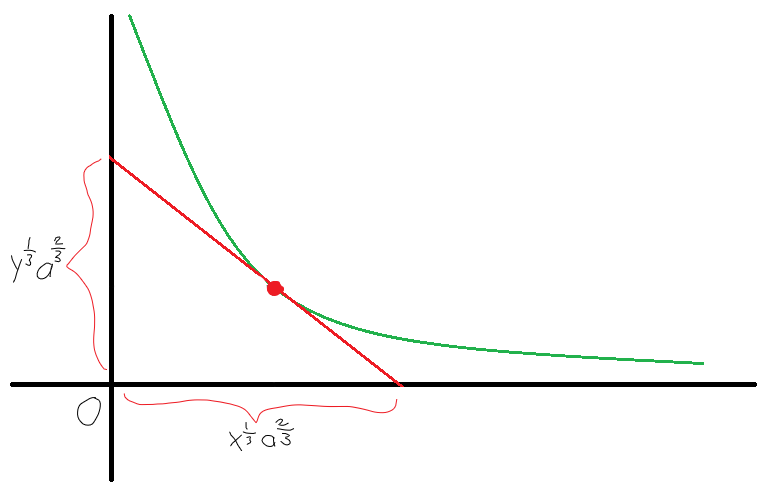
\includegraphics[width=6cm]{Q1Image(1).png}}
    \caption{Triangle formed by tangent line}
    \end{figure}
\end{minipage}\\\\
\begin{align}
    c^2 &= a^2 + b^2 \\
    c &= \sqrt{a^2 + b^2} \\
    c &= \sqrt{\left(x_0^{\frac{1}{3}}a^{\frac{2}{3}}\right)^2 + \left(y_0^{\frac{1}{3}}a^{\frac{2}{3}}\right)^2} \qquad \xleftarrow[\text{$a=x_0^{\frac{1}{3}}a^{\frac{2}{3}}$, $b=y_0^{\frac{1}{3}}a^{\frac{2}{3}}$}]{\text{sub in}}\\
    c &= \sqrt{x^{\frac{2}{3}} a^{\frac{4}{3}} + y^{\frac{2}{3}} a^{\frac{4}{3}}} \\
    c &= \sqrt{a^{\frac{4}{3}} \left( x^{\frac{2}{3}} + y^{\frac{2}{3}} \right)} \\
    c &= \sqrt{a^{\frac{4}{3}} \left( a^{\frac{2}{3}}\right)} \qquad \xleftarrow[x^{\frac{2}{3}} + y^{\frac{2}{3}} = a^{\frac{2}{3}}]{\text{sub in the equation of asteroid given from question}}\\
    c &= \sqrt{a^{\frac{6}{3}}} \\
    c &= \sqrt{a^{2}} \\
    c &= a
\end{align}
The length of the tangent line can only be positive because length is a positive magnitude - it is also given in the question that $a \in \mathbb{R^+}$. Since the length of the tangent equals $a$ and $a$ is a constant, we have finished our proof. \\

More specifically, we can say that since the asteroid is in the form $x^{\frac{2}{3}} + y^{\frac{2}{3}} = a^{\frac{2}{3}}$ and $a$ is the radius of the asteroid, not only is the length of the asteroid a constant but also it equals the radius of the asteroid.\\

\textbf{Therefore, the length of the asteroid is a constant.}






\newpage

%% PROBLEM 2
\item Gravel is being dumped from an overhead conveyor belt at a rate of 30 ft$^3$/min, and its coarseness is such that it forms a pile in the shape of a cone whose base diameter and height are always equal. Determine at what rate the height of the pile is increasing when the pile itself is 10ft high.\\

\textbf{Solution:}\\
Height = Diameter = 2 $ \times$ radius $\Longrightarrow$ Radius = $\dfrac{\text{Height}}{2}$.\\\\
Volume = $\pi r^2 \dfrac{h}{3} = \pi \left(\dfrac{h}{2}\right)^2 \dfrac{h}{3} = \dfrac{\pi}{12}h^3$.\\

We have that,
\setcounter{equation}{0}
\begingroup
\addtolength{\jot}{0.5em}
\begin{align}
    v(t) &=  \dfrac{\pi}{12}[h(t)]^3 \\
    v(t)' &= \dfrac{\pi}{12} (3) [h(t)]^2 h(t)' \\
    v(t)' &= \dfrac{\pi}{4} [h(t)]^2 h(t)' \\
    h(t)' &= \dfrac{4v(t)'}{\pi [h(t)]^2}
\end{align}
\endgroup
Since $v(t)'$ is the rate at which the volume is increasing by, we know that $v(t)' = 30$ ft$^3$/min. We also know that $h=10$ ft. Sub in the corresponding values of $v(t)'$ and $h(t)$ into line (3) to determine $h(t)'$,
\begin{align}
    h(t)' &= \dfrac{4(30)}{\pi (10)^2} \\
    h(t)' &= \dfrac{6}{5\pi} \\
    h(t)' &\approx 0.38197186
\end{align}
\textbf{Therefore, the rate of which the pile of gravel is increasing when the pile is 10ft high is 0.382 ft/min.}



\newpage

%% PROBLEM 3
\item Estimate $2.0001^5$ by using a linear approximation.\\

\textbf{Solution:}\\
Let $f(x)=x^5$ and consider the value $a = 2$ such that $f(a) = 2^5$. We can see that $f(a) = 2^5$ is much easier to calculate compared to $2.0001^5$ and will yield an output that is very close to $2.0001^5$. Recall that the equation of linear approximation is
$$L(x) = f(a) + f'(a)(x-a)$$
where $f(a)$ is a known value for some $a$ ``close" to $x$.

Let's determine all relevant values for the method of linear approximation.\\

Determine $f(a)$,
\setcounter{equation}{0}
\begin{align}
    f(a) &= a^5 \\
    f(2) &= 2^5 \\
    f(2) &= 32
\end{align}
Determine $f'(a)$,
\begin{align}
    f'(a) &= a^5 \\
    f'(a) &= 5a^4 \\
    f'(2) &= 5(2)^4 \\
    f'(2) &= 5(16) \\
    f'(2) &= 80
\end{align}
Now that we have that $f(x) = x^5$, $f(a) = f(2) = 2^5 = 32$, $f'(a) = f'(2) = 80$ and $x=2.0001$, we can determine an approximation for $2.0001^5$ using linear approximation.
\begin{align}
    L(x) &= f(a) + f'(a)(x-a) \\
    L(2.001) &= f(2) + f'(2)(2.0001-2) \\
    L(2.001) &= (32) + (80)(0.0001) \\
    L(2.001) &= 32.008
\end{align}\\
\textbf{Therefore, using linear approximation, we have that $2.0001^5 \approx 32.008$.}




\newpage

%% PROBLEM 4
\item Given that $f$ and $g$ are twice differentiable functions with second derivatives never equal to zero, if $f$ and $g$ are positive, increasing, concave up functions on an interval $A$, prove that the product $fg$ is also concave up on $A$.\\

\textbf{Solution:}\\
\setcounter{equation}{0}
Consider function $h(x)=fg$. Determine the derivative of $fg$,
\begin{align}
    h(x) &= f(x)\times g(x) \\
    h'(x) &= f'(x)g(x)+f(x)g'(x)
\end{align}
Determine the second derivative of $fg$,
\begin{align}
    h''(x) &= f''(x)g(x)+f'(x)g'(x)+f'(x)g'(x)+f(x)g''(x) \\
    h''(x) &= f''(x)g(x)+2f'(x)g'(x)+f(x)g''(x)
\end{align}
Since $f(x)$ and $g(x)$ are \textbf{increasing} and are \textbf{concave up} on $A$, we have that $f'(x) > 0$ and $g'(x) > 0$ and $f'(x)$, $g'(x)$ are both increasing on $A$ (definition 5.1, pg. 252). Similarly, since $f(x)$ and $g(x)$ are concave up, we have that $f''(x) > 0$ and $g''(x) > 0$ (theorem 5.1, pg. 252).\\

Since $f(x)$,$g(x)$,$f'(x)$,$g'(x)$,$f''(x)$ and $g''(x)$ are all positive, we have that $h''(x)$ is also positive.\\

Recall Theorem 5.1, pg. 252 states ``If $f(x) > 0$ on $I$, then the graph of $f$ is concave up on $I$". Since $h''(x) > 0$, we have that $h(x) = fg$ is concave up by Theorem 5.1, pg. 252.\\

\textbf{Therefore, the product $fg$ is concave up on $A$.}




\newpage

%% PROBLEM 5
\item Use Newton's Method to determine the positive root of the equation $\sin(x)=x^2$ to \underline{6 decimal places}.\\

\textbf{Solution:}\\
\setcounter{equation}{0}
\setcounter{figure}{0}
Recall the equation for Newton's Method of approximating roots is $x_{n+1} = x_n - \dfrac{f(x_n)}{f'(x_n)}$.\\

Firstly, in order to solve for the root using Newton's Method, we need to rewrite the equation $\sin(x)=x^2$ in the form $f(x)=0$,
\begin{align}
    \sin(x) &= x^2 \\
    0 &= x^2-\sin(x)
\end{align}
We can see that the equation on line (2) is just $y=x^2-\sin(x)$ at $y=0$, therefore, $\sin(x)=x^2$ as a function is $y=x^2-\sin(x)$.\\

Now, let's determine the derivative of $y = x^2-\sin(x)$,
\begin{align}
    y &= x^2-\sin(x) \\
    \dfrac{dy}{dx} &= 2x - \cos(x)
\end{align}
We can now write the general formula for Newton's Method by subbing in relevant values,
$$x_{n+1} = x_n - \dfrac{x_n^2-\sin(x_n)}{2x_n - \cos(x_n)}$$
\begin{minipage}{0.5\textwidth}
    Since we are not given an initial guess nor an interval to find the root, we can draw a graph to have a rough idea on what a good initial guess might be. In order to draw a graph, we need to rewrite the equation $0 = x^2-\sin(x)$ as a function.\\
    
    Looking at the graph of $y=x^2-\sin(x)$ on the right (Figure 1), we can see that the function has two roots. Since the function has two roots, our initial guess needs to be closer to the root we are interested in, otherwise we might end up approximating the wrong root.\\
    
    We can see that the first root is at $x=0$ and the second root is close to $x=1$. Since we are only interested in the positive root, we will use $x_0=1$ as our initial guess for Newton's Method.
\end{minipage}
\begin{minipage}{0.5\textwidth}
    \begin{figure}[H] %% figure 1
    \centering{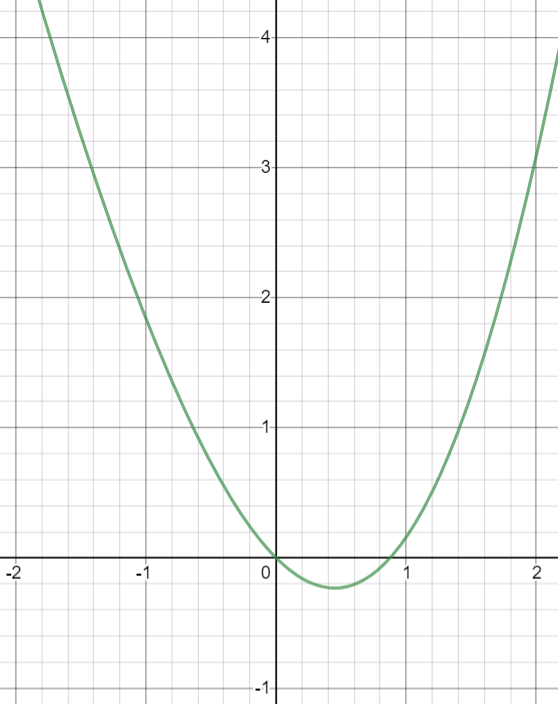
\includegraphics[width=6cm]{Q5Image.png}}
    \caption{Graph of $y=x^2-\sin(x)$}
    \end{figure}
\end{minipage}\\\\

Now that we have the general formula for Newton's Method to be $x_{n+1} = x_n - \dfrac{x_n^2-\sin(x_n)}{2x_n - \cos(x_n)}$ and\\

a specific value for our initial guess, we can begin approximating the root of $\sin(x)=x^2$ using Newton's Method.\\\\
\newpage    %% ==============   NEW PAGE   ================
First approximation at $n=0$ and $x_0 = 1$,
\begin{align}
    x_{1} &= (1) - \dfrac{(1)^2-\sin(1)}{2(1) - \cos(1)} \\
    x_{1} &= 0.891396
\end{align}
Second approximation at $n=1$ and $x_1 = 0.891396$,
\begin{align}
    x_{2} &= (0.891396) - \dfrac{(0.891396)^2-\sin(0.891396)}{2(0.891396) - \cos(0.891396)} \\
    x_{2} &= 0.876985
\end{align}
Third approximation at $n=2$ and $x_2 = 0.876985$,
\begin{align}
    x_{3} &= (0.876985) - \dfrac{(0.876985)^2-\sin(0.876985)}{2(0.876985) - \cos(0.876985)} \\
    x_{3} &= 0.876726
\end{align}
Fourth approximation at $n=3$ and $x_3 = 0.876726$,
\begin{align}
    x_{4} &= (0.876726) - \dfrac{(0.876726)^2-\sin(0.876726)}{2(0.876726) - \cos(0.876726)} \\
    x_{4} &= 0.876726
\end{align}
Since the root on the fourth approximation remained the same as the root on the third approximation (to 6 decimal places), we can stop approximating and assume that the solution is $x_{4} = 0.876726$.\\

\textbf{Therefore, using Newton's Method, the positive root of the equation $\sin(x)=x^2$ is approximately $0.876726$.}




\end{enumerate}
\end{document} 
